\documentclass[../main.tex]{subfiles}
\begin{document}
	
	\graphicspath{{AppendixD/}}
	\chapter{Supplementary Material on "Antagonism between substitutions in $\beta$-lactamase explains a path not taken in the evolution of bacterial drug resistance"}
	\label{ch:caz-supp-info}
	
    \textit{The work in this appendix is published in: Brown, C.A., Hu, L., Sun, Z., Patel, M.P., Singh, S., Porter, J.R., Sankaran, B., Venkataram Prasad, B.V.V., Bowman, G.R., Palzkill, T., Antagonism between substitutions in $\beta$-lactamase explains a path not taken in the evolution of bacterial drug resistance, J.Biol., Chem., 2020, doi:10.1074/jbc.RA119.012489} \cite{brown_antagonism_2020} \\

\section{Supplementary Data}
    
    \begin{table}[]
    \centering
    \caption{Table S1. X-ray crystallography data collection and refinement statistics for CTX-M-14 mutant enzymes. *Values in parentheses represent the highest-resolution bin.}
    \label{tab:ch2-supptable1}
    \resizebox{\textwidth}{!}{\begin{tabular}{|l|l|l|l|l|l|l|}
    \hline
                                  & P167S/D240G & E166A/D240G & E166A/P167S/ & E166A/D240G- & E166A/P167S/ & E166A/P167S/ \\ \hline
                                  &             &             & D240G        & CTX          & D240G-CTX-1  & D240G-CTX-2  \\ \hline
    PDB ID                        & 6V5E        & 6V6P        & 6V6G         & 6V7T         & 6V83         & 6V8V         \\ \hline
    Data collection               &             &             &              &              &              &              \\ \hline
    Space group                   & P 41 21 2   & P 41 21 2   & P 32 2 1     & P 21         & P 41 21 2    & P 32 2 1     \\ \hline
    a, b, c ()                & 42.2, 42,2, 261.6 & 41.9, 41.9, 259.2 & 41.4, 41.4, 231.1 & 45.1, 107.3, 47.8 & 42.4, 42.4, 262.7 & 41.3, 41.3, 231.6 \\ \hline
    $\alpha$, $\beta$, $\gamma$ (°)               & 90, 90, 90        & 90, 90, 90        & 90, 90, 120       & 90, 99.9, 90      & 90, 90, 90        & 90, 90, 120       \\ \hline
    Resolution Range (&#197;)      & 41.70 - 2.30      & 39.89 - 1.55      & 35.88 - 1.50      & 35.48 - 1.34      & 41.82 - 1.80      & 32.44 - 1.80      \\ \hline
                              & (2.38 - 2.30)     & (1.61 - 1.55)     & (1.56 - 1.50)     & (1.39 - 1.34)     & (1.84 - 1.80)     & (1.87 - 1.80)     \\ \hline
    R-merge (\%)                  & 8.4 (12.1)  & 9.7 (18.7)  & 5.6 (46.5)   & 4.7 (11.8)   & 9.4 (60.6)   & 8.7 (11.8)   \\ \hline
    I/sigma                       & 17.4 (9.6)  & 16.6 (10.3) & 30.8 (5.1)   & 17.1 (8.5)   & 31.3 (5.4)   & 11.7 (4.8)   \\ \hline
    Multiplicity                  & 7.0 (6.4)   & 11.8 (14.0) & 8.4 (10.6)   & 3.7 (3.7)    & 16.7 (19.9)  & 4.8 (2.0)    \\ \hline
    Completeness (\%)             & 88.3        & 85.5        & 98.8         & 99.4         & 100          & 97.9         \\ \hline
    Wilson B-factor ($\AA{}^2$)          & 29.4        & 10.3        & 12.1         & 9.1          & 18.2         & 14.1         \\ \hline
                                  &             &             &              &              &              &              \\ \hline
    Refinement                    &             &             &              &              &              &              \\ \hline
    Molecules per asymmetric unit & 1           & 1           & 1            & 2            & 1            & 1            \\ \hline
    No. of unique reflections & 10104 (880)       & 30051 (2829)      & 37869 (3494)      & 99523 (9924)      & 23526 (2299)      & 21924 (1871)      \\ \hline
    R-work/R-free (\%)        & 18.5 / 25.1       & 16.8 / 19.4       & 18.3 / 21.7       & 14.3 / 16.1       & 17.1 / 20.8       & 14.9 / 18.9       \\ \hline
    No. of protein residues       & 263         & 263         & 260          & 526          & 261          & 260          \\ \hline
    Ramachandran                  &             &             &              &              &              &              \\ \hline
    Favored (\%)                  & 98.5        & 98.1        & 97.7         & 98.1         & 98.5         & 98.1         \\ \hline
    Outliers (\%)                 & 0           & 0           & 0.39         & 0.38         & 0            & 0.39         \\ \hline
    Average B-factor ($\AA{}^2$)         & 31          & 14.2        & 21.2         & 14.1         & 23.3         & 16.6         \\ \hline
    Protein                       & 30.8        & 12.4        & 19.6         & 11.7         & 21.1         & 14.4         \\ \hline
    Ligand                        & -           & 23.4        & 37.3         & 18.6         & 62.2         & 28.7         \\ \hline
    Solvent                       & 34.7        & 29.1        & 32.1         & 26.7         & 36.3         & 30.2         \\ \hline
    RMS deviations                &             &             &              &              &              &              \\ \hline
    Bond length ($\AA{}$)               & 0.003       & 0.011       & 0.007        & 0.006        & 0.006        & 0.011        \\ \hline
    Bond angles (°)               & 0.685       & 1.16        & 0.92         & 0.93         & 0.96         & 1.204        \\ \hline
    \end{tabular}}
    \end{table}

\section{Supplementary Figures}

    \begin{figure}[!htb] %Positioning code for figure
        \centering
        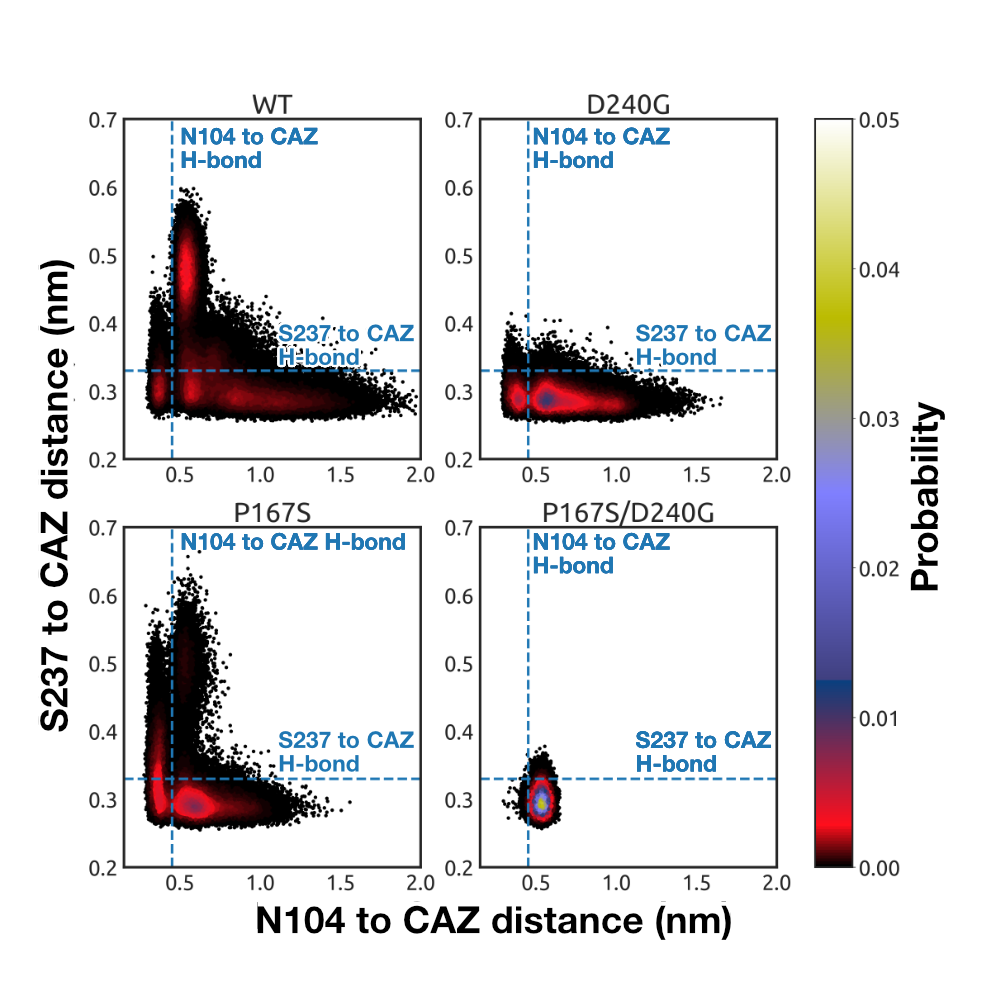
\includegraphics[width=5.5in]{ch2-suppfig1.png}
        \caption[The $\beta$3 loop and Asn104 contact CAZ in the single mutants.]{The $\beta$3 loop and Asn104 contact CAZ in the single mutants. Joint distributions of two hydrogen-bonding distances that capture the contacts between CTX-M and ceftazidime (CAZ) in the acyl-enzyme complex: i) Asn104 to the imino group of ceftazidime and ii) the backbone nitrogen of S237 on the $\beta$3 loop to the $\beta$-Lactam carbonyl oxygen of ceftazidime. Distance cutoffs for hydrogen-bonding interactions are marked (dashed lines) to indicate whether or not an interaction occurs. Distributions are shown for wild type (top left), D240G (top right), P167S (bottom left), and P167S/D240G (bottom right). Each point represents a snapshot from the molecular dynamics simulations colored according to its probability based on a 2D histogram.}
        \label{fig:ch2-suppfig1}
    \end{figure} 

    \begin{figure}[!htb] %Positioning code for figure
        \centering
        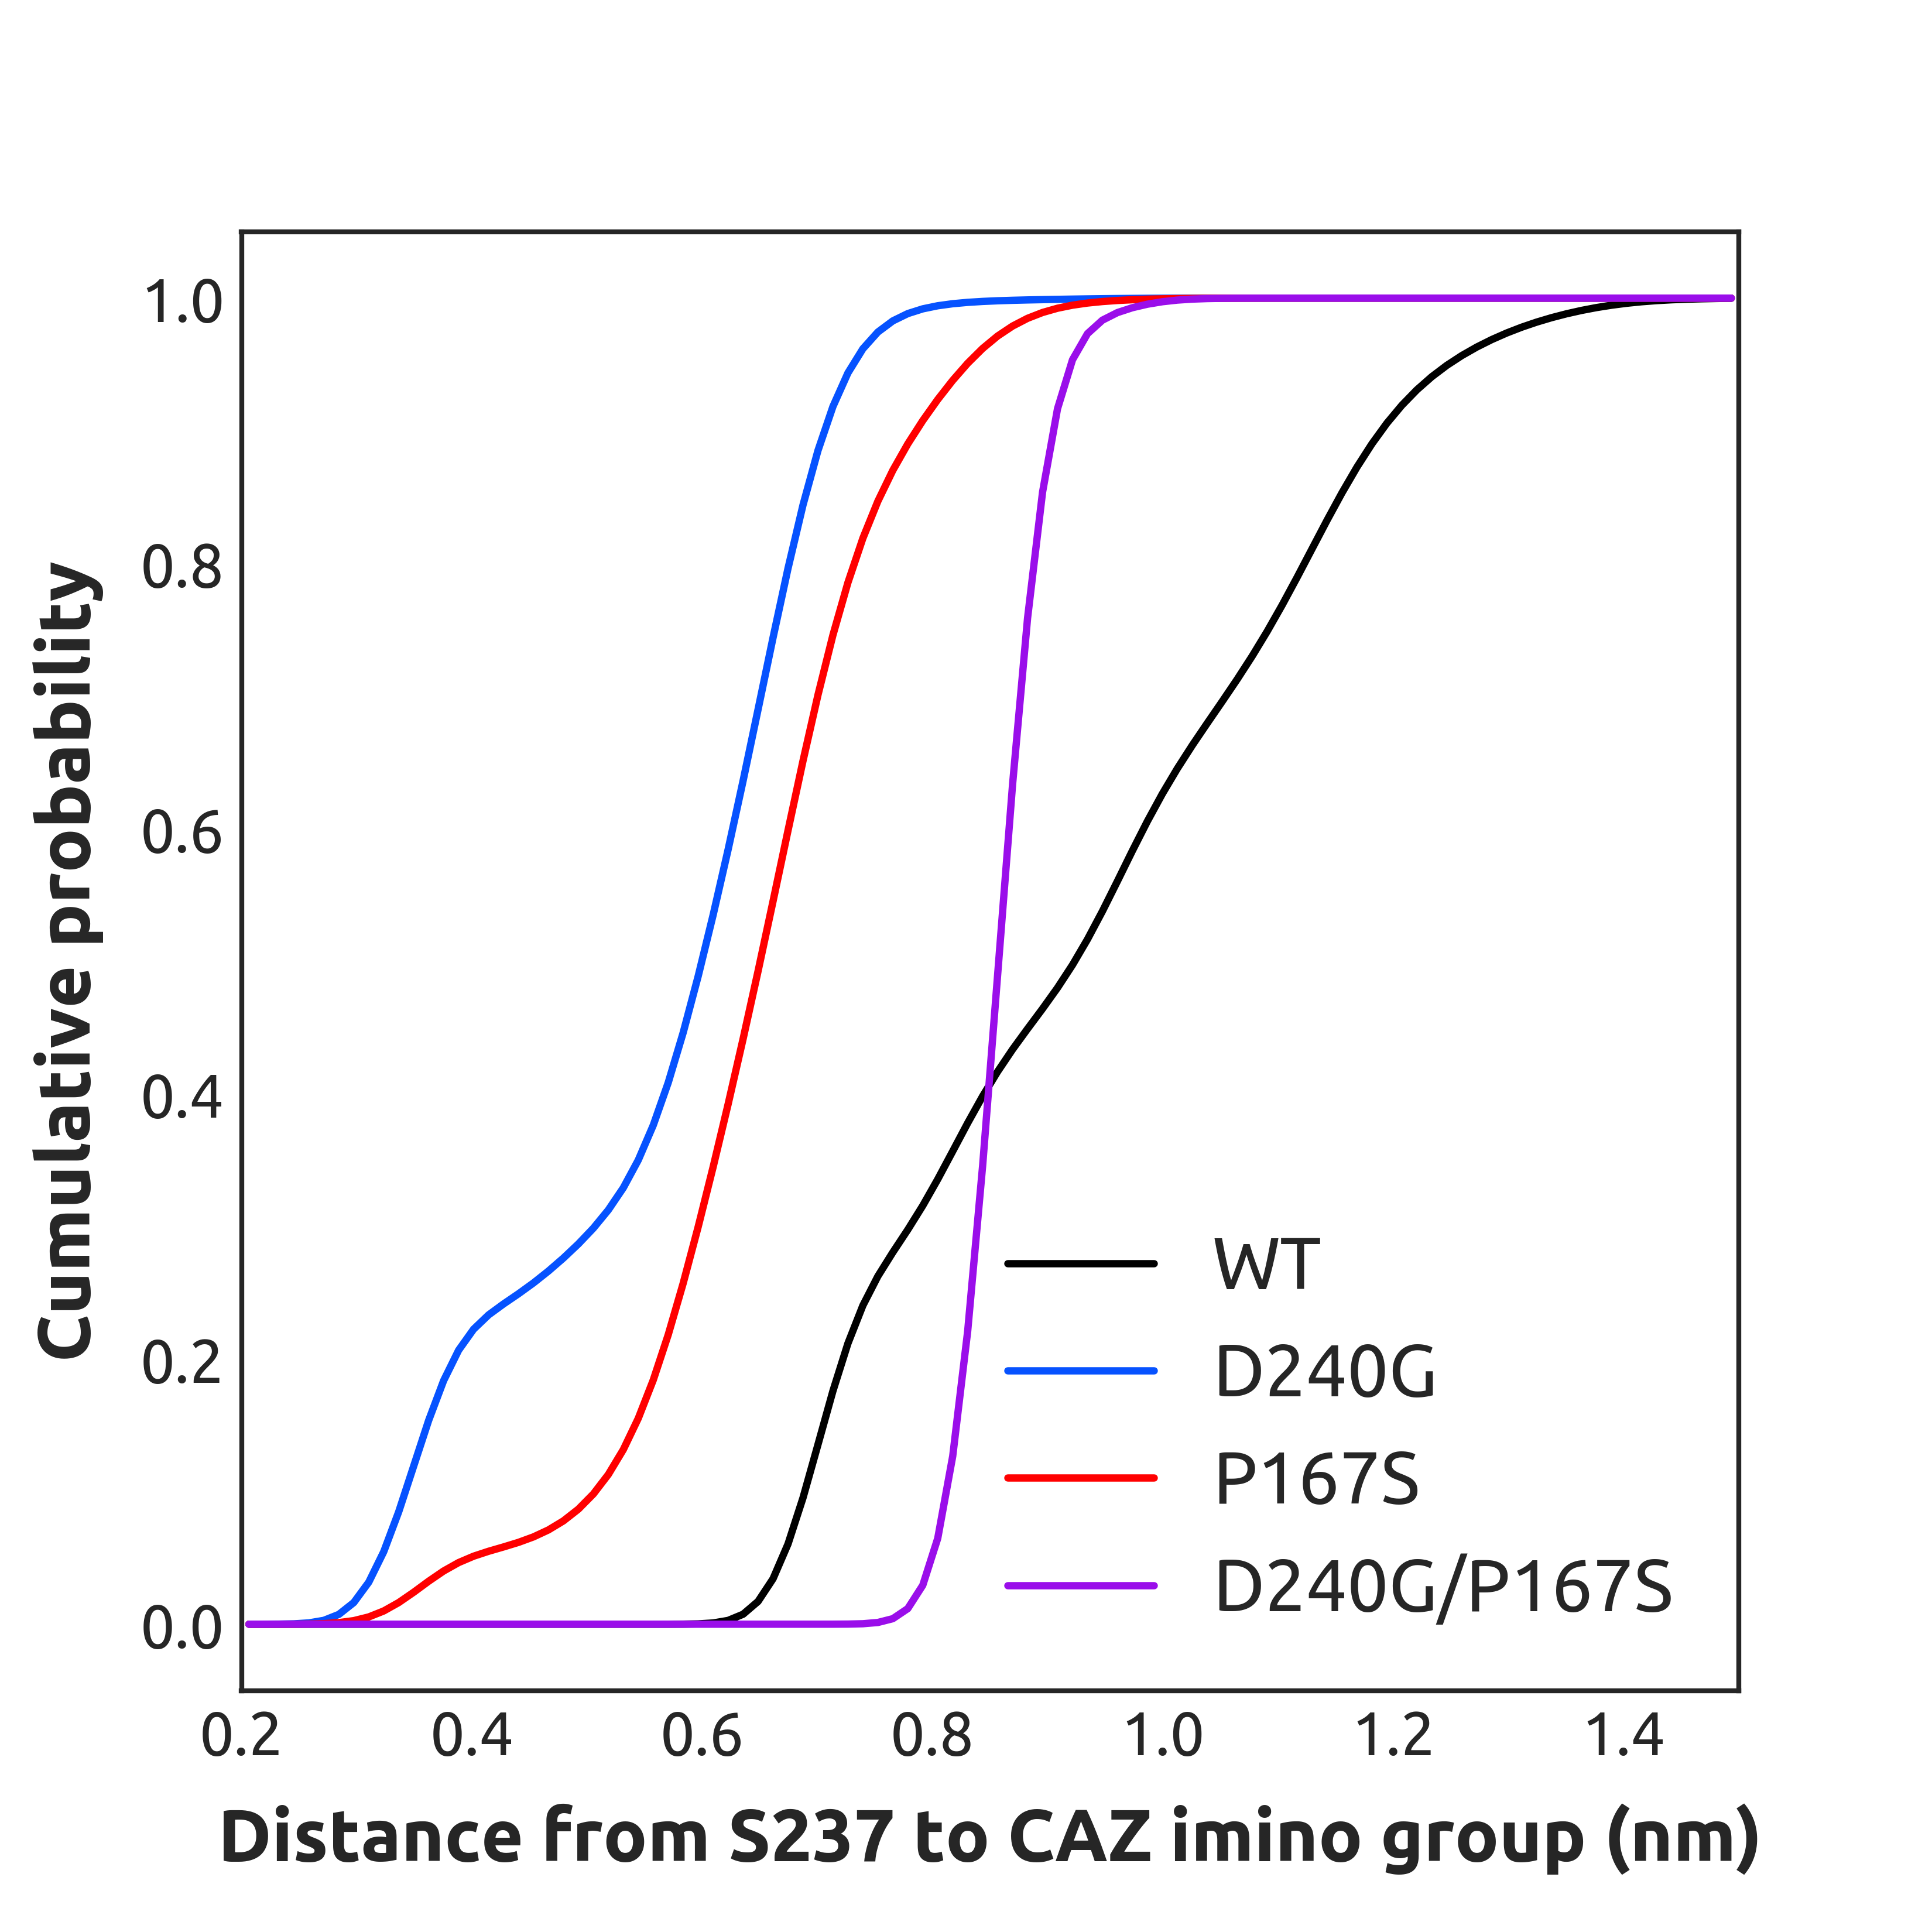
\includegraphics[width=5in]{ch2-suppfig2.png}
        \caption[Ser237 makes contacts with the imino group of ceftazidime.]{Ser237 makes contacts with the imino group of ceftazidime. Cumulative distance distribution of the sidechain oxygen of Ser237 to the carboxylate of the imino group of ceftazdime in the acyl-enzyme complex. Distributions are shown for wild type (black), D240G (blue), P167S (red), and P167S/D240G (purple).}
        \label{fig:ch2-suppfig2}
    \end{figure} 

    \begin{figure}[!htb] %Positioning code for figure
        \centering
        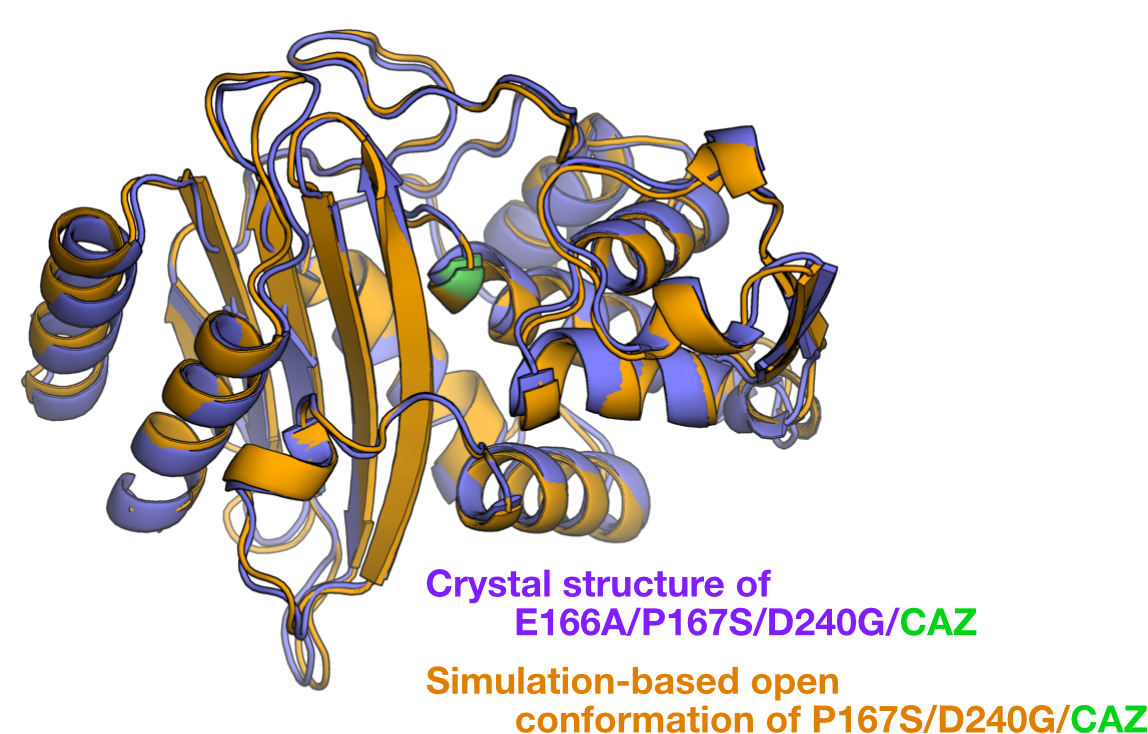
\includegraphics[width=5in]{ch2-suppfig3.png}
        \caption[MD simulations of the closed conformation of P167S/D240G capture an open conformation of the $\Omega$-loop.]{MD simulations of the closed conformation of P167S/D240G capture an open conformation of the $\Omega$-loop. Overlay of the crystal structure of E166A/P167S/D240G/CAZ (purple, Ser70 colored in green) with a representative conformation from simulation of the open conformation of the $\Omega$-loop (orange, Ser70 colored in green) sampled from simulations of the P167S/D240G variant starting from the closed conformation. In both constructs the catalytic serine that forms the acyl-enzyme complex with the serine that binds ceftazidime (labelled CAZ) is colored green. The ceftazidime molecule is not shown for clarity.}
        \label{fig:ch2-suppfig3}
    \end{figure} 
	
	
\end{document}